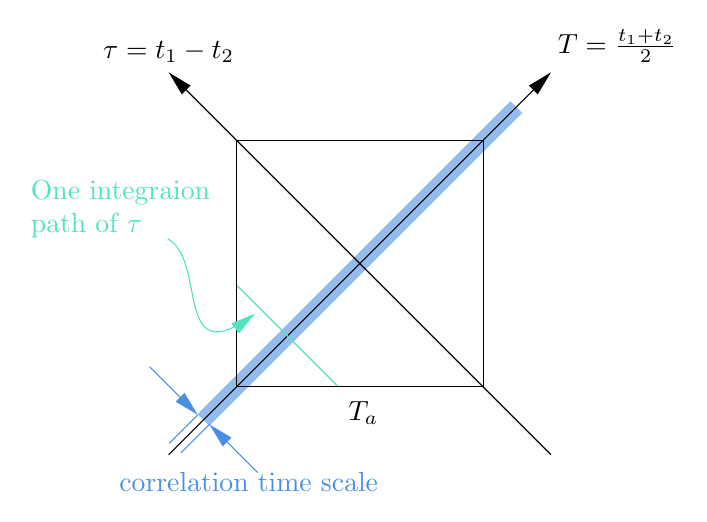
\begin{tikzpicture}[x=0.75pt,y=0.75pt,yscale=-1,xscale=1]
    %uncomment if require: \path (0,315); %set diagram left start at 0, and has height of 315
    
    %Straight Lines [id:da29302887512641407] 
    \draw [color={rgb, 255:red, 74; green, 144; blue, 226 }  ,draw opacity=0.6 ][line width=6]    (84.01,260.82) -- (234.82,110.01) ;
    %Shape: Square [id:dp3965860496444462] 
    \draw   (100,126) -- (218.83,126) -- (218.83,244.83) -- (100,244.83) -- cycle ;
    %Straight Lines [id:da10692747482044185] 
    \draw    (67.3,277.54) -- (250.12,94.71) ;
    \draw [shift={(251.54,93.3)}, rotate = 135] [fill={rgb, 255:red, 0; green, 0; blue, 0 }  ][line width=0.08]  [draw opacity=0] (12,-3) -- (0,0) -- (12,3) -- cycle    ;
    %Straight Lines [id:da4651029928641668] 
    \draw    (251.54,277.54) -- (68.71,94.71) ;
    \draw [shift={(67.3,93.3)}, rotate = 45] [fill={rgb, 255:red, 0; green, 0; blue, 0 }  ][line width=0.08]  [draw opacity=0] (12,-3) -- (0,0) -- (12,3) -- cycle    ;
    %Straight Lines [id:da12570083559205503] 
    \draw [color={rgb, 255:red, 74; green, 144; blue, 226 }  ,draw opacity=1 ]   (81.33,258.33) -- (67.61,272.06) ;
    %Straight Lines [id:da8653694800743532] 
    \draw [color={rgb, 255:red, 74; green, 144; blue, 226 }  ,draw opacity=1 ]   (87,262.94) -- (73.28,276.67) ;
    %Straight Lines [id:da2534623004469161] 
    \draw [color={rgb, 255:red, 74; green, 144; blue, 226 }  ,draw opacity=1 ]   (58.15,235.15) -- (79.92,256.92) ;
    \draw [shift={(81.33,258.33)}, rotate = 225] [fill={rgb, 255:red, 74; green, 144; blue, 226 }  ,fill opacity=1 ][line width=0.08]  [draw opacity=0] (12,-3) -- (0,0) -- (12,3) -- cycle    ;
    %Straight Lines [id:da3424301928975353] 
    \draw [color={rgb, 255:red, 74; green, 144; blue, 226 }  ,draw opacity=1 ]   (88.41,264.36) -- (110.19,286.13) ;
    \draw [shift={(87,262.94)}, rotate = 45] [fill={rgb, 255:red, 74; green, 144; blue, 226 }  ,fill opacity=1 ][line width=0.08]  [draw opacity=0] (12,-3) -- (0,0) -- (12,3) -- cycle    ;
    %Straight Lines [id:da9266881802278928] 
    \draw [color={rgb, 255:red, 80; green, 227; blue, 194 }  ,draw opacity=1 ]   (100.33,196.08) -- (148.61,244.35) ;
    %Curve Lines [id:da5722891533132757] 
    \draw [color={rgb, 255:red, 80; green, 227; blue, 194 }  ,draw opacity=1 ]   (66.94,173.52) .. controls (86.08,184.08) and (69.34,238.42) .. (107.82,210.4) ;
    \draw [shift={(109,209.52)}, rotate = 143.13] [fill={rgb, 255:red, 80; green, 227; blue, 194 }  ,fill opacity=1 ][line width=0.08]  [draw opacity=0] (12,-3) -- (0,0) -- (12,3) -- cycle    ;
    
    % Text Node
    \draw (253.54,89.9) node [anchor=south west] [inner sep=0.75pt]    {$T=\frac{t_{1} +t_{2}}{2}$};
    % Text Node
    \draw (67.3,89.9) node [anchor=south] [inner sep=0.75pt]    {$\tau =t_{1} -t_{2}$};
    % Text Node
    \draw (161.19,250.48) node [anchor=north] [inner sep=0.75pt]    {$T_{a}$};
    % Text Node
    \draw (42.33,284.67) node [anchor=north west][inner sep=0.75pt]  [color={rgb, 255:red, 74; green, 144; blue, 226 }  ,opacity=1 ] [align=left] {correlation time scale};
    % Text Node
    \draw (-0.33,143.97) node [anchor=north west][inner sep=0.75pt]  [color={rgb, 255:red, 80; green, 227; blue, 194 }  ,opacity=1 ] [align=left] {One integraion \\path of $\displaystyle \tau $};
    
    
    \end{tikzpicture}
    